% last modified 2012-06-06 by cgm

\documentclass[12pt]{article}

\usepackage{amscd}
\usepackage{xspace}
\usepackage{amsmath}
\usepackage{amsfonts}
\usepackage{amssymb}
\usepackage{amsthm}
\usepackage{graphicx}
%\usepackage{pstricks}
\usepackage{makeidx}
\usepackage{color}
\usepackage{url,hyperref}
\usepackage{fancyvrb}
\usepackage{showlabels}

\definecolor{dbluecolor}{rgb}{0,0,0.6}
\definecolor{dredcolor}{rgb}{.5,0.0,0.0}
\definecolor{dgreencolor}{rgb}{0,0.4,0}
\definecolor{blue}{rgb}{.02, .02, .908}
\newcommand{\dred}{\color{dredcolor}\bf}
\newcommand{\dblue}{\color{dbluecolor}\bf}
\newcommand{\dgreen}{\color{dgreencolor}\bf}
\def\red#1{\textcolor{red}{#1}}
\def\blue#1{\textcolor{blue}{#1}}
\def\magenta#1{\textcolor{magenta}{#1}}

\newif\ifcomments
%comment in appropriate as desired
\commentstrue
%\commentsfalse

\ifcomments
\newcommand{\djp}[1]{\magenta{DP: #1}}
\newcommand{\wdj}[1]{\red{DJ: #1}}
\newcommand{\cgm}[1]{\blue{CGM: #1}}
\else
\newcommand{\djp}[1]{}
\newcommand{\wdj}[1]{}
\newcommand{\cm}[1]{}
\fi

\def\rrr{\mathbb{R}}
\def\ccc{\mathbb{C}}
\def\zzz{\mathbb{Z}}
\def\nnn{\mathbb{N}}
\def\pf{{\bf proof}:\ }
\def\qed{$\Box$}

\newcommand{\SAGE}{{\dgreen {\sf Sage}}\xspace}
\newcommand{\sage}{\SAGE}
\newcommand{\python}{{\dblue {\sf Python}}\xspace}
\newcommand{\sympy}{{\sf SymPy}\xspace}

\newtheorem{theorem}{Theorem}
\newtheorem{corollary}[theorem]{Corollary}
\newtheorem{conjecture}[theorem]{Conjecture}
\newtheorem{lemma}[theorem]{Lemma}
\newtheorem{proposition}[theorem]{Proposition}
\newtheorem{definition}[theorem]{Definition}
\newtheorem{example}[theorem]{Example}
\newtheorem{axiom}{Axiom}
\newtheorem{remark}{Remark}
\newtheorem{exercise}{Exercise}[section]


%%%putting in some macros to simplify notation
\newcommand{\Hcal}{{\mathcal{H}}}
\newcommand{\onef}{(-1)^f}

\newcommand{\wt}{\mathop{wt}}
\newcommand{\Sum}{\sum\limits}


\begin{document}


\author{Charles Celerier, David Joyner, Caroline Melles, David
  Phillips\thanks{USNA, Mathematics Department;
email: charles.celerier@gmail.com, wdj@usna.edu (corresponding author),
cgg@usna.edu, dphillip@usna.edu}}

\title{On the Hadamard transform of monotone Boolean functions}

\maketitle

\begin{abstract}
  Let $f:GF(2)^n \rightarrow GF(2)$ be a monotone Boolean function.  Associated to
  $f$ is the Cayley graph $X$ whose vertices correspond to points of $GF(2)$
  and whose edges correspond to pairs of vectors $(v,w)$ whose sum is in
  the support of $f$.  The spectrum of $X$ (the set of eigenvalues of its
  adjacency matrix) can be computed in terms of the Hadamard transform
  of $f$.  We show that if $f$ is atomic, the adjacency matrix of $X$ is
  singular if and only if the support of $f$ has an even number of
  elements.  We ask whether it is true that for every even monotone
  function the adjacency matrix of the Cayley graph must be singular.
  We give an example in dimension $n=6$ to show that the answer to this
  question is no.  We use Sage to compute some examples of monotone
  Boolean functions, their Cayley graphs, and the graph spectra.  We
  include some interesting characterizations of monotone functions.
  We give some conditions on a monotone function that imply that the
  function is not bent.  Finally, we ask whether it is true that no
  even monotone function is bent.
\end{abstract}

\section{Introduction}

We begin with notation and by recalling some background
from \cite{art:s07}, \cite{art:bc99}.

For a given positive integer $n$ we may identify a Boolean function

\[
f:GF(2)^n\to GF(2),
\]
with its support

\[
\Omega_f = \{x\in GF(2)^n\ |\ f(x)=1\}.
\]
For each $S\subset GF(2)^n$, let $\overline{S}$ denote the
set of complements $\overline{x}=x+(1,\dots,1)\in GF(2)^n$,
for $x\in S$, and let $\overline{f}=f+1$ denote the complementary
Boolean function. Note that

\[
\Omega_f^c=\Omega_{\overline{f}},
\]
where $S^c$ denotes the complement of $S$ in $GF(2)^n$
Let

\[
\omega=|\Omega_f|
\]
denote the cardinality of the support.
We call a Boolean function {\it even} (resp., {\it odd}) if
$\omega_f$ is even (resp., odd).
We may identify a vector in $GF(2)^n$ with its support, or,
if it is more convenient, with the corresponding integer in
$\{0,1, \dots, 2^n-1\}.$ Let

\[
b:\{0,1, \dots, 2^n-1\} \to GF(2)^n
\]
be the binary representation ordered with least significant
bit last (so that, for example, $b(1)=(0,\dots, 0, 1)\in GF(2)^n$).
For convenience, we index vectors starting at 0, i.e., so a vector $x
\in GF(2)^3$ has components $x_0$, $x_1$, and $x_2$.
% Let

% \[
% \chi: 2^{\{1, 2, \dots, n\}} \to GF(2)^n,
% \]
% be the map which sends a subset $S\subset \{1,2,\dots,n\}$ to
% the vector $\chi(S)$ whose support is $S$.


Let $H_n$ denote the $2^n\times 2^n$ Hadamard matrix
defined by $(H_n)_{i,j} = (-1)^{b(i)\cdot b(j)}$, for each $i,j$
such that $0\leq i,j\leq n-1$. Inductively, these can be defined by

\[
H_1 =
\left(
\begin{array}{cc}
1 & 1\\
1 & -1 \\
\end{array}
\right),
\ \ \ \ \ \
H_n =
\left(
\begin{array}{cc}
H_{n-1} & H_{n-1}\\
H_{n-1} & -H_{n-1} \\
\end{array}
\right),
\ \ \ \ \
n>1.
\]
The {\it Hadamard transform} of $f$ is defined to be
the vector in $\rrr^{2^n}$ whose $k$th component is
\[
(\Hcal f)(k) = \sum_{i \in \{0,1,\ldots,2^n-1\}}(-1)^{b(i) \cdot b(k) + f(b(i))} =
(H_n \onef)_k,
\]
where we define $\onef$ as the column vector where the $i$th
component is
\[
\onef_i = (-1)^{f(b(i))},
\]
for $i = 0,\ldots,2^n-1$.
% $ (f(b(i))\ |\ 0\leq i\leq 2^n-1)^t$ having coordinates
% in $\{0,1\}\subset \zzz$.
We define a Boolean function
$f:GF(2)^n\to GF(2)$ to be {\it bent} if the absolute value of each
component of its
Hadamard transform is $2^{n/2}$. Clearly, since each component of the Hadamard
transform must be an integer, there are no bent functions
when $n$ is odd.

\djp{Please review the definition}

\begin{example}[a bent, odd function]
  Let $f: GF(2)^2 \rightarrow GF(2)$ be defined as $f(x_1,x_2) = x_1
  x_2$. Then $\Omega_f = \{(1,1)\}$ so $\omega = 1$ and $f$ is odd.
  Also, $f$ is bent because
  \[
  \onef =
  \begin{pmatrix}
    1 \\ 1 \\ 1 \\ -1
  \end{pmatrix}
  \]
  and so
  \[
  \Hcal f = H_2 \onef =
  \begin{pmatrix}
    1 & 1 & 1 & 1\\1 & -1 & 1 & -1\\1 & 1& -1 & -1\\
    1 & -1 & -1 & 1
  \end{pmatrix}
  \begin{pmatrix}
    1 \\ 1 \\ 1 \\ -1
  \end{pmatrix}
  =
  \begin{pmatrix}
    2 \\ 2 \\ 2 \\ -2
  \end{pmatrix}.
  \]
\end{example}

\begin{example}
\label{example:3vars}
A Boolean function of three variables cannot be bent. Let $f$ be
defined by:
%\vskip .1in
\begin{center}
\begin{tabular}{c|cccccccc}
$x_1$                    & 0 & 0 & 0 & 0 & 1 & 1 & 1 & 1 \\
$x_2$                    & 0 & 0 & 1 & 1 & 0 & 0 & 1 & 1 \\
$x_3$                    & 0 & 1 & 0 & 1 & 0 & 1 & 0 & 1 \\ \hline
$\onef$                  & 1 & -1 & 1 & -1 & 1 & -1 & 1 & -1   \\
${\mathcal{H}}f$   & 0 & 8 & 0 & 0 & 0 & 0 & 0 & 0    \\
\end{tabular}
\end{center}

This function is even because
\[
\Omega_f = \{ (0,0,1),  (0,1,1),  (1,0,1),  (1,1,1) \},\ \mbox{ so } \
\omega = 4.
\]

\end{example}

\begin{example}
\label{example:4vars}
A Boolean function of four variables:

%\vskip .1in
\begin{center}
\begin{tabular}{c|cccccccc cccccccc}
$x_1$                    & 0 & 0 & 0 & 0 & 0 & 0 & 0 & 0 & 1 & 1 & 1 & 1 & 1 & 1 & 1 & 1\\
$x_2$                    & 0 & 0 & 0 & 0 & 1 & 1 & 1 & 1 & 0 & 0 & 0 & 0 & 1 & 1 & 1 & 1\\
$x_3$                    & 0 & 0 & 1 & 1 & 0 & 0 & 1 & 1 & 0 & 0 & 1 & 1 & 0 & 0 & 1 & 1\\
$x_4$                    & 0 & 1 & 0 & 1 & 0 & 1 & 0 & 1 & 0 & 1 & 0 & 1 & 0 & 1 & 0 & 1\\ \hline
$(-1)^f$                        & 1 & 1  & 1  & 1  & 1   & 1 & 1 & -1  & 1 & 1 & 1 & -1 & -1 & -1 & -1 & -1 \\
${\mathcal{H}}f$   & 4 & 4 & 4 & -4 & 8 & 0 & 0 & 0 & 8 & 0 & 0 & 0 & -4 & -4 & -4 & 4  \\
\end{tabular}
\end{center}
In this example, the function is even and $\omega = 6$.
\end{example}

\cgm{Changed $f$ to $(-1)^f$.6/4/12}

% Let $V = GF(2)^n$ and let $W = GF(2)^{2^n-1}$. Let
% $b:\{0,1,...,2^n-1\} \to V$ be the
% binary representation, with least significant bit last. Regard the
% list of vectors $b(i)$, $i\geq 0$, as columns of a $n\times 2^n$
% matrix $B'$ and let $B$ be the submatrix of non-zero columns.
% The matrix $B$ is $n \times (2^n-1)$ and may also be regarded as the parity check
% matrix of the $[2^n-1, n, 3]$ binary Hamming code $C \subset W$.

% Let $f:GF(2)^n \to GF(2)$ be a Boolean function
% of the variables $x_0,x_1,\dots, x_{n-1}$.
% It is not hard to characterize the set of Boolean functions which
% have the property that (a) the $n$ subfunctions
% $f(0,x_1,\dots, x_{n-1})$, \dots, $f(x_0,\dots, x_{n-2},0)$
% have a given parity pattern\footnote{For example, the pattern could
% be that all are even, in the sense that
% each such subfunction has the property that their support has
% an even number of elements.}, (b) $f(0) = 0$.

% To be concrete, let us see what it means for a Boolean function
% $f$ to have the property that each of the
% subfunctions

% \[
% f|_{x_0=1}, \ \ \ f|_{x_1=1}, \ \ \ \dots, \ \ \ f|_{x_{n-1}=1},
% \]
% is odd (where each is regarded as a Boolean function in the same $n-1$
% variables). The idea is as follows:

% \begin{itemize}
% \item
%  regard $f$ as a vector $w_f$ in $W$ by ignoring the $1$st coordinate (which
% is $0$, by assumption (b)),
% \item
% assume that $f|_{x_0=0}$, $f|_{x_1=0}$, \dots, $f|_{x_{n-1}=0}$ all have odd
% support. This is equivalent to the statement

% \[
%                     B w_f = (1, 1, ..., 1) \in V.
% \]
% \item
%  The vectors $v$ for which $B\cdot v = 0$ is the Hamming code $C$. In
% other words, $C$ is the pre-image of the zero vector under $H$. Every
% other pre-image  (e.g., that of the all $1$s vector) is a coset of
% $C$. Which one? Let $e = (0, ..., 0, 1) \in W$ and
% note $B\cdot e = (1, ..., 1) \in V$.
% (In the terminology of error-correcting codes,
% $(1, ..., 1) \in V$ is our syndrome and $e = (0, ..., 0, 1) \in W$
% is our coset leader.)

% Getting back to our Boolean function $f$, we see that the above
% subfunctions are all odd if and only if $w_f \in C+e$.
% \end{itemize}


For any two $x,y \in GF(2)^{n}$,
let $d(x,y)$ denote the {\it Hamming metric}:

\begin{equation}
d(x,y)=|\{0\leq i\leq n-1\,\,|\,\,
x_{i}\not=y_{i}\}|.
\end{equation}
We define the {\it weight} ${\rm wt}$ of $x$ to be the number
of non-zero coordinates of $x$, so $d(x,y)={\rm wt}(x-y)$.


\begin{example}
We use Sage to look at the example of
\[
f(x_0,x_1,x_2,x_3) = x_0x_1x_2 + x_0x_1x_3 + x_0x_2x_3 + x_0x_2 +
x_1x_2x_3 + x_1x_2 + x_2x_3.
\]
First, we attach the file {\tt afsr.sage} available from Celerier
\cite{url:c12},
then run the following commands.

%\vskip .15in

\begin{Verbatim}[fontsize=\scriptsize,fontfamily=courier,fontshape=tt,frame=single,label=\sage]

sage: from sage.crypto.boolean_function import *
sage: R.<x0, x1, x2, x3> = BooleanPolynomialRing(4)
sage: f = BooleanFunction(x0*x1*x2 + x0*x1*x3 + x0*x2*x3 + x0*x2 +
x1*x2*x3 + x1*x2 + x2*x3)
sage: g = BooleanFunction([0,0,0,0,0,1,1,1,0,0,0,1,1,1,1,1])
sage: g.is_bent()
False
sage: is_monotone(g)
True
sage: g.truth_table(format='int')
(0, 0, 0, 0, 0, 1, 1, 1, 0, 0, 0, 1, 1, 1, 1, 1)
sage: f.truth_table(format='int')
(0, 0, 0, 0, 0, 1, 1, 1, 0, 0, 0, 1, 1, 1, 1, 1)
sage: g.algebraic_normal_form()
x0*x1*x2 + x0*x1*x3 + x0*x2*x3 + x0*x2 + x1*x2*x3 + x1*x2 + x2*x3
sage: f.algebraic_normal_form()
x0*x1*x2 + x0*x1*x3 + x0*x2*x3 + x0*x2 + x1*x2*x3 + x1*x2 + x2*x3

\end{Verbatim}

%\vskip .2in
\noindent
This shows how to construct Boolean functions in Sage using
the {\tt sage.crypto} module. The only command from {\tt afsr.sage} is
the {\tt is\_monotone} function\footnote{Monotonicity is defined in \S
  3 below.}. We then show that, in spite of $f$ and
$g$ being constructed in different ways, they have the same values
(``truth table'') and have the same algebraic normal form\footnote{The
  ANF is discussed, for example, in \cite{thesis:c12}.}.

\end{example}



\section{The Cayley graph}

Let $X=(V,E)$ be the {\it Cayley graph} of $f$:

\[
V = GF(2)^n,\ \ \ \ E = \{(v,w)\in V\times V\ |\ f(v+w)=1\}.
\]
We shall assume throughout and without further mention that

\[
f(0)\not=1,
\]
so $X$ has no loops.
In this case, $X$ is an $\omega$-regular graph having $r$ connected
components, where

\[
r = |GF(2)^n/{\rm Span}(\Omega_f)|.
\]
For each vertex $v\in V$, the set of neighbors $N(v)$ of $v$ is given
by

\[
N(v)=v+\Omega_f,
\]
where $v$ is regarded as a vector and the addition is induced by the
usual vector addition in $GF(2)^n$.
Let $A = (A_{ij})$ be the $2^n\times 2^n$ adjacency matrix of
$X$, so

\[
A_{ij} = f(b(i)+b(j)),
\ \ \ \ \ 0\leq i,j\leq 2^n-1.
\]

\begin{example}
\label{example:3vars-graph}
Here are some Sage commands to help visualize the
Boolean function $f$ of three variables in
Example \ref{example:3vars}:

%\vskip .15in

\begin{Verbatim}[fontsize=\scriptsize,fontfamily=courier,fontshape=tt,frame=single,label=\sage]

    sage: flist = [0,1,0,1,0,1,0,1]
    sage: V = GF(2)^3
    sage: Vlist = V.list()
    sage: f = lambda x: GF(2)(flist[Vlist.index(x)])
    sage: X = boolean_cayley_graph(f, 3)
    sage: X.adjacency_matrix()
    [0 1 0 1 0 1 0 1]
    [1 0 1 0 1 0 1 0]
    [0 1 0 1 0 1 0 1]
    [1 0 1 0 1 0 1 0]
    [0 1 0 1 0 1 0 1]
    [1 0 1 0 1 0 1 0]
    [0 1 0 1 0 1 0 1]
    [1 0 1 0 1 0 1 0]
    sage: X.spectrum()
    sage: X.show(layout="circular")

\end{Verbatim}

The last command gives rise to the Cayley graph $X$ of $f$ shown in
Figure \ref{fig:monotone-boolean-fcns-3vars-graph}.
The adjacency matrix $A$ of $X$ is given by

\begin{figure}[t!]
\begin{minipage}{\textwidth}
\begin{center}
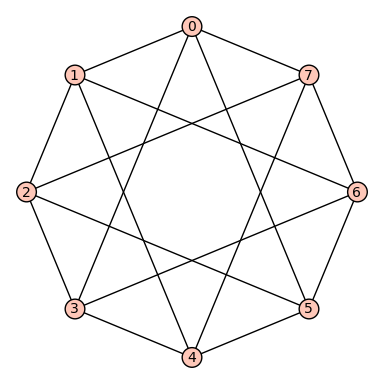
\includegraphics[height=5cm,width=5cm]{monotone-boolean-fcns-3vars-graph}
\end{center}
\end{minipage}
\caption{The Cayley graph of the Boolean function of three
  variables from Example \ref{example:3vars}. (The vertices are
  ordered as in the Example.)}
\label{fig:monotone-boolean-fcns-3vars-graph}
\end{figure}



\[
A =
\left(\begin{array}{rrrrrrrr}
0 & 1 & 0 & 1 & 0 & 1 & 0 & 1 \\
1 & 0 & 1 & 0 & 1 & 0 & 1 & 0 \\
0 & 1 & 0 & 1 & 0 & 1 & 0 & 1 \\
1 & 0 & 1 & 0 & 1 & 0 & 1 & 0 \\
0 & 1 & 0 & 1 & 0 & 1 & 0 & 1 \\
1 & 0 & 1 & 0 & 1 & 0 & 1 & 0 \\
0 & 1 & 0 & 1 & 0 & 1 & 0 & 1 \\
1 & 0 & 1 & 0 & 1 & 0 & 1 & 0
\end{array}\right)
\]
and the graph spectrum by

\[
\{-4, 0, 0, 0, 0, 0, 0, 4\}.
\]

\end{example}


\begin{example}
\label{example:4vars-graph}
For the Boolean function of four variables in
Example \ref{example:4vars}, the Cayley graph
is given in Figure \ref{fig:monotone-boolean-fcns-4vars-graph}.
The adjacency matrix $A$ of the graph is

% sage: flist = [0,0,0,0,0,0,0,1,0,0,0,1,1,1,1,1]
% sage: V = GF(2)^4
% sage: Vlist = V.list()
% sage: f = lambda x: GF(2)(flist[Vlist.index(x)])
% sage: X = boolean_cayley_graph(f, 4)
% sage: X.show(layout="circular")
% sage: X.show(layout="circular", dpi=200)

\begin{figure}[t!]
\begin{minipage}{\textwidth}
\begin{center}
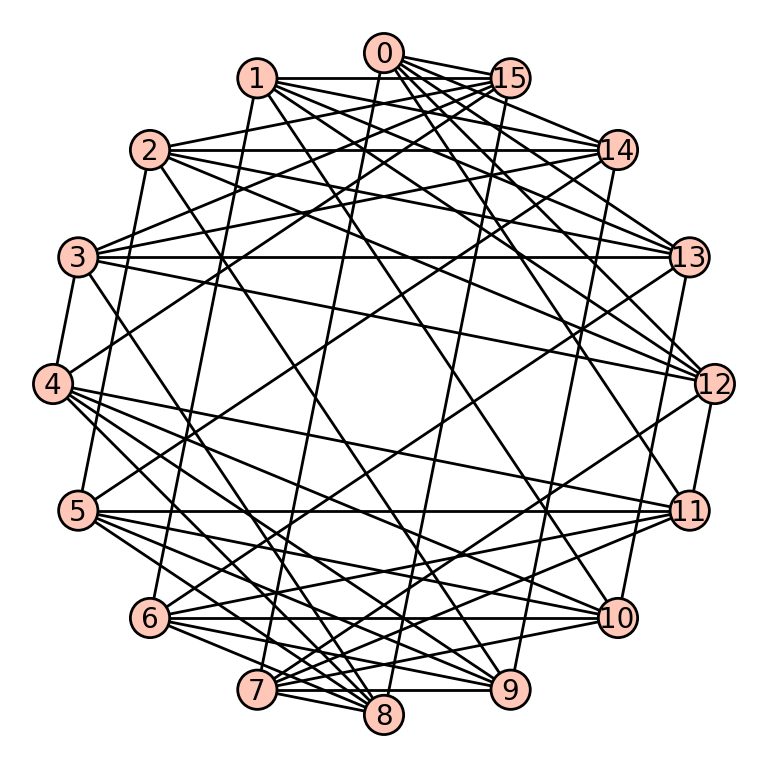
\includegraphics[height=9cm,width=9cm]{monotone-boolean-fcns-4vars-graph}
\end{center}
\end{minipage}
\caption{The Cayley graph of the Boolean function of four
  variables from Example \ref{example:4vars}. (The vertices are
  ordered as in the Example.)}
\label{fig:monotone-boolean-fcns-4vars-graph}
\end{figure}

{\small{
\[
A =
\left(\begin{array}{rrrrrrrrrrrrrrrr}
0 & 0 & 0 & 0 & 0 & 0 & 0 & 1 & 0 & 0 & 0 & 1 & 1 & 1 & 1 & 1 \\
0 & 0 & 0 & 0 & 0 & 0 & 1 & 0 & 0 & 0 & 1 & 0 & 1 & 1 & 1 & 1 \\
0 & 0 & 0 & 0 & 0 & 1 & 0 & 0 & 0 & 1 & 0 & 0 & 1 & 1 & 1 & 1 \\
0 & 0 & 0 & 0 & 1 & 0 & 0 & 0 & 1 & 0 & 0 & 0 & 1 & 1 & 1 & 1 \\
0 & 0 & 0 & 1 & 0 & 0 & 0 & 0 & 1 & 1 & 1 & 1 & 0 & 0 & 0 & 1 \\
0 & 0 & 1 & 0 & 0 & 0 & 0 & 0 & 1 & 1 & 1 & 1 & 0 & 0 & 1 & 0 \\
0 & 1 & 0 & 0 & 0 & 0 & 0 & 0 & 1 & 1 & 1 & 1 & 0 & 1 & 0 & 0 \\
1 & 0 & 0 & 0 & 0 & 0 & 0 & 0 & 1 & 1 & 1 & 1 & 1 & 0 & 0 & 0 \\
0 & 0 & 0 & 1 & 1 & 1 & 1 & 1 & 0 & 0 & 0 & 0 & 0 & 0 & 0 & 1 \\
0 & 0 & 1 & 0 & 1 & 1 & 1 & 1 & 0 & 0 & 0 & 0 & 0 & 0 & 1 & 0 \\
0 & 1 & 0 & 0 & 1 & 1 & 1 & 1 & 0 & 0 & 0 & 0 & 0 & 1 & 0 & 0 \\
1 & 0 & 0 & 0 & 1 & 1 & 1 & 1 & 0 & 0 & 0 & 0 & 1 & 0 & 0 & 0 \\
1 & 1 & 1 & 1 & 0 & 0 & 0 & 1 & 0 & 0 & 0 & 1 & 0 & 0 & 0 & 0 \\
1 & 1 & 1 & 1 & 0 & 0 & 1 & 0 & 0 & 0 & 1 & 0 & 0 & 0 & 0 & 0 \\
1 & 1 & 1 & 1 & 0 & 1 & 0 & 0 & 0 & 1 & 0 & 0 & 0 & 0 & 0 & 0 \\
1 & 1 & 1 & 1 & 1 & 0 & 0 & 0 & 1 & 0 & 0 & 0 & 0 & 0 & 0 & 0
\end{array}\right)
\]
}}
and the graph spectrum is

\[
\{ -4, -4, -2, -2, -2, 0, 0, 0, 0, 0, 0, 2, 2, 2, 2, 6\}.
\]
These may be computed using Sage commands, as in the last example.


\end{example}


% Let $w_k\in \{\pm 1\}^{2^n}$ be the column vector whose
% $i$th component is

% \[
% (w_k)_i = (w_k)_v = (-1)^{b(k)\cdot v},
% \ \ \ \ \ \
% v = b(i)\in GF(2)^n.
% \]
% Here we abuse notation and use both $i\in \{0,1,\dots, 2^n-1\}$
% and the corresponding vector $v=b(i)\in GF(2)^n$ as subscripts. For
% $k=0,\ldots,2^n-1$,
% \begin{eqnarray*}
% (Aw_k)_v & =& \sum_{x\in v+\Omega_f}  (-1)^{b(k)\cdot x}\\
%  & =&  \sum_{x\in \Omega_f}  (-1)^{b(k)\cdot v} (-1)^{b(k)\cdot x}\\
%  & =&  (-1)^{b(k)\cdot v} \sum_{x\in GF(2)^n}  (-1)^{b(k)\cdot
%    x}f(x)\\
%  & = & w_k (H_n \chi(f))_k,
% %%following is no longer correct as \Hcal f \not= \sum_{x \in GF(2)^n
% %%(-1)^{b(k)\cdot x}
% %% & =& (w_k)_v ({\mathcal{H}}f) (b(k)),
% \end{eqnarray*}
\cgm{I rewrote the following section, changing notation and adding some subscripts.6/4/12}

We wish to relate the spectrum of the Cayley graph $X$ (the eigenvalues of the adjacency matrix $A$) to the Hadamard transform $\mathcal H f = 
H_n (-1)^f$.  Recall that $(-1)^f$ is defined to be the column vector whose 
$i$th component is $((-1)^f)_i=(-1)^{f_i}$, where $f_i=f(b(i))$ for 
$i = 0, 1, ... , 2^n-1$.  Note that $f$ and $(-1)^f$ are related by the 
equation 
$$f=\frac 1 2 (e - (-1)^f),$$
where $e=(1,1,...,1)$.  
For $k=0, 1, ... , 2^n-1$, let $w_k\in \{\pm 1\}^{2^n}$ be the column vector whose
$i$th component is
\[
(w_k)_i = (-1)^{b(k)\cdot b(i)}.
\]
Each vector $w_k$ is an eigenvector of $A$, since for 
each $i$, 
\begin{eqnarray}
\nonumber (Aw_k)_i & =& \sum_{j=0}^{2^n-1} f(b(i)+b(j))(-1)^{b(k) \cdot b(j)}\\
\nonumber & =& (-1)^{b(k) \cdot b(i)} \sum_{j=0}^{2^n-1}(-1)^{b(k) \cdot (b(i)+b(j))} f(b(i)+b(j)) \\
\nonumber & =& (w_k)_i \sum_{l=0}^{2^n-1} (-1)^{b(k) \cdot b(l)}f(b(l))\\
%\nonumber  (Aw_k)_i & =& \sum_{x\in b(i)+\Omega_f}  (-1)^{x \cdot b(k)}\\
%\nonumber & =&  \sum_{x\in \Omega_f}  (-1)^{b(i)\cdot b(k)} (-1)^{x \cdot b(k)}\\
%\nonumber & =&  (-1)^{b(i)\cdot b(k)} \sum_{x\in GF(2)^n}  (-1)^{x \cdot b(k)}f(x)\\
\nonumber & =& (w_k)_i \sum_{l=0}^{2^n-1} (H_n)_{k,l} f_l\\
\label{eq:w1} & =& (w_k)_i (H_n f)_k \\
\nonumber  & =& (w_k)_i (H_n \frac 1 2 (e - \onef))_k\\
\label{eq:w2} & =& (w_k)_i \frac{1}{2} (H_n e - \Hcal f)_k.
%%following is no longer correct as \Hcal f \not= \sum_{x \in GF(2)^n
%%(-1)^{b(k)\cdot x}
%% & =& (w_k)_v ({\mathcal{H}}f) (b(k)),
\end{eqnarray}
%where $f \in \{0,1\}^{2^n}$ is defined where
%$f_i = f(b(i))$,
%for $i \in \{1,\ldots,2^n\}$. Note that $f_i = \frac{1 - (-1)^f_i}{2}$.
Then Equation \eqref{eq:w1} proves that $w_k$ is an eigenvector of $A$ having eigenvalue
%%$\lambda_k =  ({\mathcal{H}}f) (b(k)).$
$\lambda_k = (H_n f)_k$, where $H_n$ is the $n$th Hadamard matrix, 
 and Equation \eqref{eq:w2} demonstrates the
affine relationship $\lambda_k =  \frac 1 2 (H_n e - \mathcal H f)_k$ between the spectrum of $X$ and the Hadamard transform.
Therefore, the spectrum of $X$,
\[
{\rm Spectrum}(X) = \{\lambda_k\ |\ 0\leq k\leq 2^n-1\},
\]
is explicitly computable as an expression in terms of $f$.

There is another useful expression for $\lambda_k$.
Let $\Omega_f^*$ be the $\omega\times n$ matrix whose column vectors
are the elements of $\Omega_f$:
\[
\Omega_f^* =
\left(
\begin{array}{c}
y_1
\hdots 
y_\omega
\end{array}
\right),
\ \ \ \ \ \ \ \
\Omega_f = \{y_1,\dots, y_\omega\}.
\]
%Let $v=b(k)$, where $0\leq k\leq 2^n-1$. We have
%not sure how the extra notation is helpful
Then, for ${k \in \{0,\ldots,2^n-1\}}$,
\begin{eqnarray*}
\lambda_k & =& \sum_{y\in GF(2)^n}  (-1)^{b(k)\cdot y}f(y)\\
 & =&  \sum_{y\in \Omega_f}  (-1)^{b(k)\cdot y}\\
 & =&  \sum_{y\in \Omega_f}  (1 - 2 (b(k)\cdot y\mod 2))\\
 & = & \omega - 2 {\rm wt}\left( \big(b(k)^\top \Omega_f^*\big) \mod 2\right),\\
\end{eqnarray*}
This tells us that an integer $m$ belongs to
$ {\rm Spectrum}(X)$ if and only if there is
an $x\in GF(2)^n$ such that
the number of $y\in \Omega_f$ which are not orthogonal mod 2 to $x$ in $GF(2)^n$ is
$\frac{m-\omega}{2}$.

\cgm{Changed row to column vectors in $\Omega_f^*$ and changed last sentence to not orthogonal mod 2. 6/6/12}
% \begin{remark}
% Here is the connection with the Laplacian spectrum.

% ??????????
% \end{remark}


\section{Monotone functions}

Define a partial order $\leq $ on $GF(2)^n$ as follows:
for each $v,w\in GF(2)^n$, we say

\[
v\leq w
\]
whenever we have
$v_1 \leq w_1$, $v_2 \leq w_2$, \dots, $v_n \leq w_n$.
%(This partial order is not to be confused with the lexicographical order.)
A Boolean function is called {\it monotone} (increasing) if whenever
we have $v\leq w$ then we also have $f(v) \leq f(w)$.  
Examples \ref{example:3vars} and 
\ref{example:4vars} above are monotone.

\cgm{Added note regarding ex.s 2 and 3. 6/6/12}

Note that if $f$ and $g$ are monotone then (a) $f+g+fg$ is also
monotone, and (b) $\overline{\Omega_f}\cap  \overline{\Omega_g}
=\overline{\Omega_{fg}}$.
(Equivalently, if $f$ and $g$ are monotone {\it decreasing} then
so is $fg$, and moreover we have $\Omega_f\cap \Omega_g
=\Omega_{fg}$.)

There are some interesting characterizations of monotone functions.

\begin{itemize}
\item
For $f:GF(2)^n \to GF(2)$ any Boolean function of $n$ variables,
let

\[
\begin{array}{c}
f_0(x_1,\dots ,x_{n-1}) = f(0,x_1,\dots ,x_{n-1}),
\ \ \ \ \ \\
f_1(x_1,\dots ,x_{n-1}) = f(1,x_1,\dots ,x_{n-1}).
\end{array}
\]
The function $f$ is monotone if and only if
(a) both of the subfunctions $f_0$ and $f_1$ are
monotone and (b) $\Omega_{f_0} \subset \Omega_{f_1}$.

\item For a given positive integer $n$ and our partial ordering, the
  {\it Hasse diagram}, $D_n$, is the directed graph with a vertex for
  each vector in $GF(2)^n$ and for which $(v,w)$ is an edge if $v\leq
  w$ and $\wt(w)=\wt(v)+1$ (see Example \ref{example:digraph}).  We
  define a {\it closure} of a directed graph $G = (V,E)$ to be a set
  of nodes without any outgoing edges, i.e., a set of nodes, $C
  \subseteq G$, with the property that if $i \in C$ and $(i,j) \in E$,
  then $j \in C$. We can then count the number of monotone functions
  on $n$ variables by counting the number of closures on
  $D_n$.\footnote{We believe this is a known result, but are not able
    to find a previous reference.} Closures on directed graphs have
  several applications, e.g., in defense \cite{art:o87}, mining
  \cite{art:j68,art:hc00,art:bz10}, and shipping \cite{art:r70}.
  \begin{theorem}
    For all positive integers $n$, the set of closures on $D_n$ are in
    one-to-one correspondence with the set of monotone functions on
    $GF(2)^n$.
  \end{theorem}
  \begin{proof}
    Let $n$ be a given positive integer and consider the set of
    monotone functions on $GF(2)^n$. We claim that the relation
    mapping Boolean functions on $GF(2)^n$ to their support defines a
    one-to-one correspondence from monotone functions to closures on
    $D_n$. Note that such a relation is a function from Boolean
    functions to subsets of $GF(2)^n$, i.e., subsets of vertices in
    $D_n$. We claim that the support of a monotone Boolean function is
    a closure on $D_n$. Let $f$ be a given monotone Boolean function
    on $GF(2)^n$. For given vertices $v,w \in GF(2)^n$, suppose that
    $v \in \Omega_f$ and that $(v,w)$ is an edge in $D_n$. Then, $w_i
    = v_i + 1$ for exactly one $i \in \{0,\ldots,2^n-1\}$ and $w_j =
    v_i$ for all $j \in \{0,\ldots,2^n-1\} \setminus \{i\}$, i.e., $v
    < w$. Then, because $v \in \Omega_f$ and $f$ is monotone, $1 =
    f(v) \leq f(w)$ so $w \in \Omega_f$. Thus, $\Omega_f$ is a closure
    in $D_n$.

    To see that the support is injective, note that two different
    Boolean functions have different supports. To see that the support
    is surjective, let $C \subseteq GF(2)^n$ be a given closure in
    $D_n$ and define $f_C$ as the function with $C$ as a set of
    support vectors, i.e., for all $v \in C$, $f_C(v) = 1$. We claim
    that $f_C$ is monotone.  Let $v, w \in GF(2)^n$ be given where $v
    \leq w$ and $v\not=w$. If $f_C(v) = 0$ then $f_C(v) \leq f_C(w)$,
    trivially, so assume that $f_C(v)=1$, i.e., $v \in C$. Note that
    if $v \leq w$ and $v\not=w$ then for some positive integer $k$,
    there are $k$ components where $v$ has a zero and $w$ has a one.
    For $i \in \{0,\ldots,2^n-1\}$, let $e_i$ denote the vector with
    one in component $i$ and zero in all other components. Then there
    is a set $\{i_1,\ldots,i_k\} \subset \{0,\ldots,2^n-1\}$ where $w
    = v+\Sum_{j=1}^k e_j$. For $\ell \in \{0,\ldots,k\}$, let $u_\ell
    = v+ \Sum_{j=1}^\ell e_j$. By the definition of the Hesse diagram,
    for $\ell \in \{0,\ldots,k-1\}$, $(v_\ell,v_{\ell+1})$ are edges
    in $D_n$. Then, as $v=v_0 \in C$, by the closure property, $v_\ell
    \in C$ for all $\ell \in \{0,\ldots,k\}$, so, in particular,
    $f_C(w) = f_C(v_k) = 1 \geq f_C(v)$.

  \end{proof}

\item The set $\{{\rm supp}(v)\ |\ \overline{v}\in\Omega_f\}$ is an
  ideal\footnote{ An {\it ideal} in a set $U$ is a collection $I$ of
    subsets of $U$ such that $B\in I$ and $A\subset B$ implies $A\in
    I$.  } of ${\{0,1,\dots,n-1\}}$ (see, for example, Kleitman
  \cite{art:k69}).

\end{itemize}

For each $v\in GF(2)^n$,
define a monotone function $f=f_v$ to be
{\it atomic based on $v$} if its support
consists of all vectors greater than $v$,
i.e., if

\[
\Omega_f = \{x\in GF(2)^n \ |\ v\leq x\},
\]
where $\leq$ is the partial order defined above.
We call $f$ {\it atomic} if there is some
$v\not= 0$ such that $f$ is atomic based on $v$.
Note that Example \ref{example:3vars} is 
monotone and atomic based on $(0,0,1)$ while Example 
\ref{example:4vars} is monotone but not atomic.

\cgm{Changed Ex 2 not atomic to Ex 2 is atomic. 6/6/12}

\begin{definition}
\label{def:leastsupport}
{\rm
Let $f:GF(2)^n \to GF(2)$ any monotone function.
We say that $\Gamma\subset GF(2)^n$ forms a set of vectors of
{\it least support} for $f$ if $\Gamma$ consists of all
vectors in $\Omega_f$ which are smallest in the
partial ordering $\leq$ on $GF(2)^n$.
}
\end{definition}

For example, the set of vectors of least support for Example \ref{example:4vars} is 
$\Gamma = \{ (0,1,1,1),(1,0,1,1),(1,1,0,0)\}$.

\cgm{Added this ref to Example 3. 6/6/12}

 A monotone function is atomic if and only if it has only one vector in
its set of least supports.
Here is an interesting group-theoretical characterization of atomic
monotone functions.
% If $W\subset GF(2)^n$, let $\overline{W}\subset GF(2)^n$ denote the subset of all complements
% $\overline{w}=(1, \dots, 1)+w$ of elements $w \in W$.

\begin{proposition}
\label{prop:atomic-subspace}
Let $f$ be a Boolean monotone function which is not a constant function.
Then $f$ has atomic support if and only if the
set of complements $\overline{\Omega_f}$ is a subspace of $GF(2)^n$.
\end{proposition}

\begin{proof}
Suppose that $f$ has atomic support based on $v$.
Then $v\leq w$ for all $w \in \Omega_f$.
Then $\overline{w}\leq \overline{v}$ for all $\overline{w} \in
\overline{\Omega_f}$.
If $\overline{w_1}$ and $\overline{w_2}$ are in $\overline{\Omega_f}$
then  $\overline{w_1}+\overline{w_2}\leq \overline{v}$.
Indeed, consider the $i$th component of
$\overline{v}$:  if it is $0$ then the $i$th components of
$\overline{w_1}$ and $\overline{w_2}$
must be $0$, and if it is $1$ then it is impossible for the $i$th
component of the sum to be any larger.  Therefore $\overline{\Omega_f}$ is a subspace.

Conversely, suppose that $\overline{\Omega_f}$ is a proper subspace of $GF(2)^n$ and
let $x$ be any element of $\overline{\Omega_f}$.

% We claim that $f(x)\not= 0$.
% Otherwise,  both $x$ and its complement $\overline{x}$ are in $\Omega_f$ so both
% $\overline{x}$ and $x$ must be in $\overline{\Omega_f}$.
% Since $\overline{\Omega_f}$ is a subspace, $x+\overline{x}=(1,1,\dots ,1) \in \overline{\Omega_f}$, so
% $(0,0,0,\dots ,0) \in \Omega_f$. Since $f$ is monotone, this imples
% that $f$ is a constant. This contradition proves the claim.

Next, we claim that if $x \in \overline{\Omega_f}$ and if $y\leq x$,
then $y \in \overline{\Omega_f}$.
But $y\leq x$ if and only if $\overline{y}\geq \overline{x}$.
Because $f$ is monotone, $\overline{y} \in \Omega_f$, proving the claim.

Now let $z$ be any element of maximal weight in $\overline{\Omega_f}$.
Let $h$ be the weight of $z$. Since $f$ is monotone, there must be at
least $h$ weight $1$ vectors in $\overline{\Omega_f}$, by the
previous claim.
Suppose there is a vector $y \in \overline{\Omega_f}$ such that $y$ is
not less than or equal to $z$.
Then there must be at least $h+1$ (distinct) weight $1$ vectors in
$\overline{\Omega_f}$.
Their sum must also be in $\overline{\Omega_f}$, so $z$ is not a
maximal weight element of $\overline{\Omega_f}$.
Therefore $\overline{\Omega_f}$ consists of all elements $y$ of $GF(2)^n$
such that $y\leq z$ and $\Omega_f$ consists of all elements $w$
such that $w\geq \overline{z}$ (namely all the complements of those $y$'s).
Therefore $\Omega_f$ is atomic based on $\overline{z}$.
\end{proof}

\begin{example}
\label{example:digraph}
Here is an example of a monotone function whose least
support vectors are given by

\[
\Gamma =\{ (1,0,0,0), (0,1,1,0), (0,1,0,1), (0,0,1,1)
\} \subset GF(2)^n.
\]

\begin{figure}[t]
\begin{center}
\begin{picture}(300,0)(0,200)
\put(150,190){\text{0000}}
%\put(160,177){\text{0}}
\put(150, 180){\vector(-3, -1){80}}
\put(155, 177){\vector(-2, -1){40}}
\put(170, 180){\vector(3, -1){80}}
\put(165, 177){\vector(2, -1){40}}
% wt = 1
\put(260,140){\text{0001}}
%\put(270,127){\text{1}}
\put(270, 127){\vector(-1, -1){25}}
\put(275, 130){\vector(1, -1){25}}
\put(267, 130){\vector(-4, -1){115}}
\put(190,140){\text{0010}}
%\put(200,127){\text{2}}
\put(198, 130){\vector(-4, -1){115}}
\put(202, 130){\vector(0, -1){25}}
\put(205, 133){\vector(3, -1){85}}
\put(100,140){\text{0100}}
%\put(110,127){\text{4}}
\put(105, 130){\vector(-3, -1){88}}
\put(115, 132){\vector(4, -1){125}}
\put(110, 130){\vector(3, -1){85}}
\put(30,140){\text{\bf{1000}}}
%\put(40,127){\text{8}}
\put(37, 127){\vector(-1, -1){25}}
\put(42, 128){\vector(1, -1){25}}
\put(50, 127){\vector(3, -1){75}}
% wt = 2
\put(300,90){\text{\bf{0011}}}
%\put(310,77){\text{0}}
\put(309, 82){\vector(-3, -1){94}}
\put(310, 82){\vector(-1, -1){30}}
\put(240,90){\text{\bf{0101}}}
%\put(250,77){\text{5}}
\put(247, 84){\vector(-4, -1){120}}
\put(252, 82){\vector(2, -3){20}}
\put(180,90){\text{\bf{0110}}}
%\put(190,77){\text{6}}
\put(188, 85){\vector(-4, -1){130}}
\put(194, 85){\vector(2, -1){67}}
\put(120,90){\text{\bf{1001}}}
%\put(130,77){\text{9}}
\put(134, 81){\vector(-1, -1){26}}
\put(137, 82){\vector(2, -1){50}}
\put(60,90){\text{\bf{1010}}}
%\put(65,77){\text{10}}
\put(72, 80){\vector(-1, -1){25}}
\put(77, 82){\vector(4, -1){118}}
\put(0,90){\text{\bf{1100}}}
%\put(5,77){\text{12}}
\put(17, 80){\vector(2, -3){19}}
\put(22, 80){\vector(3, -1){84}}
% wt = 3
\put(260,40){\text{\bf{0111}}}
%\put(270,27){\text{7}}
\put(280, 36){\vector(-4, -1){108}}
\put(190,40){\text{\bf{1011}}}
%\put(195,27){\text{11}}
\put(207, 36){\vector(-2, -1){46}}
\put(100,40){\text{\bf{1101}}}
%\put(105,27){\text{13}}
\put(108, 36){\vector(2, -1){46}}
\put(30,40){\text{\bf{1110}}}
%\put(35,27){\text{14}}
\put(40, 36){\vector(4, -1){110}}
% wt = 4
\put(150,-5){\text{\bf{1111}}}
%\put(155,-17){\text{15}}
\end{picture}\\[3.0in]
\end{center}
\caption{{\bf{Bold font}} means the Boolean function takes the value $1$ at that point in $GF(2)^4$.
Regular font means the function is $0$. This is another way of drawing
the Hasse diagram for the four-dimensional unit hypercube.}
\end{figure}
This example has the property that the function
$f(x_0,x_1,x_2,x_3)$ is even (i.e., the support
$\Omega_f$ has an even number of elements),
yet the subfunctions
$f(x_0,0,x_1,x_2)$, $f(x_0,x_1,0, x_2)$, $f(x_0,x_1,x_2,0)$
are all odd, but $f(0,x_0,x_1,x_2)$ is even.
\end{example}


Here is a compact algebraic form that these
monotone functions must take.  We use the multinomial notation 
$x^v=x_1^{v_1}x_2^{v_2}...x_n^{v_n}$.

\djp{I stopped editing here (outside of moving Caroline's example to
  this section) as I was not sure what $x^v$ is when $x$ is a vector.
  Is this defined somewhere?} 
\cgm{added explanation of $x^v$ 6/6/12}

\begin{theorem}
\label{theorem:compact-alg-form}
Let $f$ be a monotone function whose least
support vectors are given by $\Gamma \subset GF(2)^n$.
Then

\[
f(x) = 1+\prod_{v\in\Gamma} (x^v+1).
\]
\end{theorem}

\begin{proof}
For $y \in GF(2)^n$, let

\[
g(y) = 1+\prod_{v\in\Gamma} (x^v+1).
\]
Let

\[
S_y = \{v\in \Gamma \ |\ v\leq y\}.
\]
Case 1: $S_y=\emptyset$. In this case, $y$ does not
meet the support of $f$, since $f$ is monotone. Moreover, we have

\[
g(y)=1+(0+1)\cdot \dots \cdot (0+1)=0.
\]
Therefore, $f(y)=0=g(y)$, as desired.

\noindent
Case 2: $S_y \not=\emptyset$. Let $m = |S_y|$.
In this case, there are $2^m$ terms in
$\prod_{v\in S_y} (y^v+1)$, all of which are non-zero.
Therefore, $f(y)=1=g(y)$, as desired.

\end{proof}

Let us regard ${f}(x) = 1+\prod_{v\in\Gamma} (x^v+1)$
as being integer-valued.  For all non-zero $y \in GF(2)^n$, the
Hadamard transform of $f$ has the following
expression:

\[
({\mathcal{H}}f)(y) =\sum_{x\in \Omega_f}  (-1)^{y \cdot x} =
\sum_{{\footnotesize{
\begin{array}{c}
x \\
{\rm supp}(v) \subseteq {\rm supp}(x) \\
{\rm some}\ v\in  \Gamma
\end{array}
}}}
(-1)^{y \cdot x}.
\]
% When it it true that
% $|{\rm supp}(v) \cap {\rm supp}(x)|$
% is even for all $x$ such that
% ${\rm supp}(v) \subset {\rm supp}(x),$
% for some $v\in  \Gamma$?

This last expression for the Hadamard transform may help answer
the following question: For which monotone functions (if any) is the graph
$X$ singular? 

\cgm{I don't understand the above, starting with Let us regard ... ending with Hadamard transform.
1.  The expression for $\mathcal H f$ doesn't agree with our new definition.  2.  I don't see how Theorem 10 
is being used.  3.  I think we want to look at $\lambda_k$ instead of $\mathcal H f (k)$.  4.  I don't see how $y$ 
nonzero is being used.  I propose the following.  6/6/12}

The $k$th element $\lambda_k$ of the spectrum of the Cayley graph $X$ is given by
\begin{eqnarray*}
\lambda_k 
 & =&  \sum_{x\in \Omega_f}  (-1)^{b(k)\cdot x}\\
 & =&  \sum_{{\footnotesize{
\begin{array}{c}
x \\
{\rm supp}(v) \subseteq {\rm supp}(x) \\
{\rm some}\ v\in  \Gamma
\end{array}
}}}
(-1)^{b(k) \cdot x}
.\\
\end{eqnarray*}
This last expression for the elements of the spectrum of $X$ may help answer
the following question: For which monotone functions (if any) is the graph
$X$ singular? 
In other words, if $f$ is monotone,
we want to characterize when $0\in {\rm Spectrum}(X)$.
We can answer this question in some special cases.
For example, the following result addresses the special case of atomic
monotone functions.

\begin{theorem}
Let $f$ be a Boolean atomic monotone function.
The associated Cayley graph is singular if and only if
$\omega$ is even.

\end{theorem}

\begin{proof}
First, note that if $\omega$ is odd then
$({\mathcal{H}}f) (y)\not= 0$ for all $y\in GF(2)^n$ for parity
reasons.
(This is true for all Boolean functions $f$ and does not even require
$f$ to be monotone.)
Therefore, we may assume $\omega$ is even.

We must show that, for some $x\in GF(2)^n$, half the vectors in
$\Omega_f$ are orthogonal to $x$ and half are not.
Assume $f = f_v$ is atomic based on $v$,
let $M\subset \{1,2,\dots, n\}$ denote the support of
$v$ and let $m=|M|$.
Consider the image of $\Omega_f$ under the
projection map

\[
p = p_M: GF(2)^n \to GF(2)^{n-m},
\]
given by puncturing all coordinates
indexed by an element of $M$,

\[
p(\Omega_f)\subset GF(2)^{n-m}.
\]
Since $f$ is monotone based on $v$, this subset is actually
``everything'':

\[
p(\Omega_f) = GF(2)^{n-m}.
\]

Pick any $x\in GF(2)^n$ whose support \cgm{6/6/12}
%is disjoint from that of $v$. 
is not contained in the support of $v$.  
This is possible as long as $v$ is not the all-ones vector,
$v\not= (1,\dots, 1)\in GF(2)^n$.
(The case of $f=f_v$ where $v= (1,\dots, 1)\in GF(2)^n$
cannot arise since we assumed $\omega$ is even.)
Note $x\in \overline{\Omega_f}$. Since $\overline{\Omega_f}$
is a subspace, by the previous proposition, it is orthogonal
to half the vectors in $\overline{\Omega_f}$ and not orthogonal
to the other half. Thus, since $\omega$ is
even, the same orthogonality property
holds if we replace $\overline{\Omega_f}$ by
$\Omega_f$.
\end{proof}

Recall that a strongly regular graph is a
regular graph $(V,E)$ with vertices $V$ and common degree $c$
for which there are also integers $d$ and $e$ such that:
\begin{itemize}
\item
every two adjacent vertices have $d$ common neighbors,
\item
every two non-adjacent vertices have $e$ common neighbors.
\end{itemize}

\begin{proposition}
Let $f:GF(2)^n\to GF(2)$ denote a monotone function for which
$v\in \Omega_f$ implies ${\rm wt}(v)>n/2$.
Then $f$ is not bent.
\end{proposition}

\begin{proof}
Suppose not. Let $\Gamma$ denote the Cayley graph of $f$, so
(since we are assuming $f$ is bent) $\Gamma$ is strongly regular
having parameters $d,e$ with $d=e$ (where $d,e$ denote the number
of common neighbors in the adjacent, non-adjacent cases).
For any vertex $v$ in $\Gamma$, let $N(v)$ denote the neighbors
(i.e., adjacent vertices) of $v$. Strongly regular implies that the cardinality

\[
|N(v)\cap N(0)|
\]
is independent of which vertex $v \in \Gamma$ we select.
(Here $0$ denotes the vertex $0\in GF(2)^n$.)
Let $v\in \Omega_f$ be a vector having lowest weight
and let $j=(1,\dots,1)\in GF(2)^n$.
Then

\[
|N(v)\cap N(0)| = |N(j)\cap N(0)| = |\overline{\Omega_f}\cap \Omega_f|=0.
\]
This implies $d=e=0$, which is a contradiction (this equality, in turn, implies
$\Omega_f=\emptyset$ by page 2 in Stanica \cite{art:s07}).
\end{proof}

Let $f$ be any even monotone function of $4$ variables. By an
exhaustive search using Sage, it can be verified that such an $f$ has
the property that there is some Walsh coefficient that is zero.
\cgm{We have not defined Walsh coefficient and I haven't found a 
good definition on the internet.  I suggest just calling this an element of 
the spectrum. 6/6/12}
In other words, its Cayley graph is singular in the sense that it
has $0$ as an eigenvalue. In particular, such a monotone function
cannot be bent.

This suggests two questions:
\begin{itemize}
\item
Is it true that for every even monotone function, the associated
Cayley graph $X$ is singular?
\item
Is it true that no even monotone function is bent?
\end{itemize}
The answer to the first question is no. In fact, Example \ref{ex:caroline}
below gives a counterexample in dimension $6$.
The second question is, as far as we know, open.


\section{Derived Boolean functions}

Let $f$ be a monotone Boolean function on $GF(2)^n$.    We define a new ``derived'' Boolean function $F$ on $GF(2)^n$ as follows.
Let $v_1$, ... , $v_r$ be the least supports of $f$.  Let $A_i$ be the atomic set generated by $v_i$, i.e., $A_i$ consists of all vectors $v$ in
$GF(2)^n$ such that $v \geq v_i$.  For $x \neq (0,0,...,0)$ in $GF(2)^n$, let $A_x$ be the intersection of all $A_i$ such that $i$ is in the support of $x$.
For example, if $x=(1,1,0,...,0)$, then $A_x=A_1 \cap A_2$.  If $x=(0,0,...,0)$, $A_x$ is is defined to be all of $GF(2)^n$.
Now we define $F(x)=0$ if $|A_x|$ is even and $F(x)=1$ if $|A_x|$ is odd.

Notice that $|A_x|$ is always a power of 2, so $F(x)=1$ if and only if $|A_x|=1$, i.e., if and only if the set $A_x$ consists of the vector
of all 1's.  If $|A_x|=1$ then $A_y=1$ for any $y \geq x$ since by
definition, $(1,1,...,1) \in A_y \subset A_x$.
Therefore the derived function $F$ is also a monotone Boolean function.  Note that $F$ may be identically 0, even though we have assumed that $f$ is not.

\begin{example}
If $F$ is the zero function then the adjacency matrix of $f$ has 0 as an eigenvalue.  To see this,
we first note that each intersection of atomic sets is atomic (as a
corollary of Proposition \ref{prop:atomic-subspace}).
(In fact, if $A$ is atomic based on $v$ and $B$ is atomic based on
$w$, then $A \cap B$ is atomic
based on $u$, where the support of $u$ is the union of the supports of
$v$ and $w$.)  Also, each atomic
set with more than one element has an equal number of vectors of even
and odd weights.
For any set $S$ of vectors in $GF(2)^n$, let
$S^-$ be the vectors in $S$ with odd weight and let $S^+$ be the set of vectors in $S$ with even weight.  Then $|A_x^+|=|A_x^-|$ for
all $x$ if $F$ is the zero function.  The support of $f$ is
$\Omega_f=\cup_i A_i$.  Using the formula for the cardinality of a
union of sets,

\begin{align*}
|A_1^+ \cup A_2^+ \cup ... \cup A_r^+|
&=\sum_{i=1}^r |A_i^+| - \sum_{i\neq j} |A_i^+ \cap A_j^+| \\
&+ \sum_{i,j,k\ {\rm distinct}} |A_i^+ \cap A_j^+ \cap A_k^+| -  \\
& \dots +(-1)^{r-1} |A_1^+ \cap A_2^+ \cap ... \cap A_r^+|\\
&=|A_1^- \cup A_2^- \cup ... \cup A_r^-|
\end{align*}
so that the number of even and odd weight vectors in $\Omega_f=\cup_i A_i$ must be equal if $F$ is the zero function.
Note that the vectors in $\Omega_f$ which are orthogonal to $(1,1,...,1)$ are exactly the even weight vectors.
Now we apply the criterion of section 2 with $m=0$ and $x=(1,1,...,1)$.   This tells us that $0$ belongs to the spectrum
of the graph of $f$ because the number of vectors in $\Omega_f$ which are orthogonal to $(1,1,...,1)$ is $\omega/2$.

\end{example}

Note that this construction can be generalized to any finite
collection of nonempty
sets $A_i$ in $GF(2)^n$ by taking $F(x)=|\Omega \cap A_x|$ mod $2$,
but the resulting
Boolean function $F$ is not necessarily monotone.  For example, if
$A_i$ consists
of all vectors whose $i$th component is $0$, then the value of $F$ on
the vector $e_i$
whose $i$th component is 1 and whose other components are 0 tells us whether the subfunction $f|_{x_i=0}$ is even or odd.

Constructing a function $g: GF(2)^n \rightarrow \zzz$ with $g(x) =
|A_x|$ (i.e., the actual
cardinality, not the cardinality mod $2$) provides some useful
counting arguments, as shown below,
which can help rule out certain integers as eigenvalues of the spectrum of the Cayley graph of $f$.

Consider an atomic set $A$ based on a vector $v$.  If $x$ is a vector
in $GF(2)^n$ with support
contained in the support of $v$, then
$x \cdot y = x \cdot v$ for all $y \in A$.  Otherwise, if the support
of $x$ is not contained in the
support of $v$, $x$ is orthogonal to exactly half the vectors in $A$.
Using this fact we can
construct, by some simple counting arguments, examples of monotone Boolean functions whose
Cayley graphs cannot have 0 in their spectra.

For example, suppose that $f$ is a monotone Boolean function on $GF(2)^n$ such that
the least support of $f$ consists of vectors $v_1$, $v_2$, and $v_3$
with $|A_1|=|A_2|=|A_3|=4$
and $|A_i \cap A_j|=1$ for $i \neq j$.  Then $|\Omega_f|=10$.  Let
$\bf{1}=(1,1,...,1)$.
For any $x$ in $GF(2)^n$, the number of vectors $y$ in $A_i$  such
that $x \cdot y=x \cdot 1$ is
either 2 or 4.  Therefore the total number of vectors $y$ in $\Omega_f
= A_1 \cup A_2 \cup A_3$
such that $x \cdot y = x \cdot 1$ is one of 4, 6, 8, or 10.  This
means that the number of
vectors in $\Omega_f$ which are orthogonal to $x$ cannot be
$\omega/2=5$ for any $x$ in
$GF(2)^n$.  Therefore the Cayley graph of $f$ cannot have $0$ in its
spectrum.

We show now in Example \ref{ex:caroline} an explicit construction of
an even, monotone boolean
function for which $0$ is not an eigenvalue.
\begin{example}
\label{ex:caroline}
Let $n=6$ and \cgm{6/6/12} let $f$ be the monotone function whose 
set of vectors of least support is 
$$\Gamma = \{ (1,1,1,1,0,0),(1,1,0,0,1,1),(0,0,1,1,1,1)\}.$$  
Using Theorem \ref{theorem:compact-alg-form}, we obtain the compact algebraic form 
\[
f(x_0,x_1,x_2,x_3,x_4,x_5) =
x_0x_1x_2x_3 + x_0x_1x_4x_5 + x_2x_3x_4x_5
.\]
This function
is monotone yet has no vanishing Walsh coefficients.  \cgm{Same comment as above - haven't defined 
Walsh coefficient. 6/6/12/}
As with the previous examples, we attach the file {\tt afsr.sage} available from Celerier
\cite{url:c12}, then run the following commands.

%\vskip .15in

\begin{Verbatim}[fontsize=\scriptsize,fontfamily=courier,fontshape=tt,frame=single,label=\sage]

sage: V = GF(2)^(6)
sage: L = [V([1,1,0,0,1,1]),V([0,0,1,1,1,1]), V([1,1,1,1,0,0])]
sage: f = monotone_from_support(L)
sage: is_monotone(f)
True


\end{Verbatim}

%\vskip .1in
\noindent
These commands simply construct a Bolean function $f$ whose least
support are the vectors in {\tt L}.
Next, we compute the Hadamard transform of this using
both the method built into Sage's {\tt sage.crypto}
module, and the function in {\tt afsr.sage}.

%\vskip .15in

\begin{Verbatim}[fontsize=\tiny,fontfamily=courier,fontshape=tt,frame=single,label=\sage]

sage: f.walsh_hadamard_transform()
(-44, -12, -12, 12, -12, 4, 4, -4, -12, 4, 4, -4, 12, -4, -4, 4, -12, 4, 4, -4, 4, 4, 4, -4,
4, 4, 4, -4, -4, -4, -4, 4, -12, 4, 4, -4, 4, 4, 4, -4, 4, 4, 4, -4, -4, -4, -4, 4, 12,
-4, -4, 4, -4, -4, -4, 4, -4, -4, -4, 4, 4, 4, 4, -4)
sage: f.algebraic_normal_form()
x0*x1*x2*x3 + x0*x1*x4*x5 + x2*x3*x4*x5
sage: x0,x1,x2,x3,x4,x5 = var("x0,x1,x2,x3,x4,x5")
sage: g = x0*x1*x2*x3 + x0*x1*x4*x5 + x2*x3*x4*x5
sage: Omega = [v for v in V if g(x0=v[0], x1=v[1], x2=v[2], x3=v[3], x4=v[4], x5=v[5])<>0]
sage: len(Omega)
10
sage: g = lambda x: x[0]*x[1]*x[2]*x[3] + x[0]*x[1]*x[4]*x[5] + x[2]*x[3]*x[4]*x[5]
sage: [walsh_transform(g,a) for a in V]
[44, 12, 12, -12, 12, -4, -4, 4, 12, -4, -4, 4, -12, 4, 4, -4, 12, -4,-4, 4, -4, -4, -4, 4,
-4, -4, -4, 4, 4, 4, 4, -4, 12, -4, -4, 4, -4, -4, -4, 4, -4, -4, -4, 4, 4, 4, 4, -4, -12,
4, 4, -4, 4, 4, 4, -4, 4, 4, 4, -4, -4, -4, -4, 4]

\end{Verbatim}

\vskip .1in
\noindent
(Note: the Walsh transform method in the {\tt BooleanFunction} class
in Sage is off by a sign from the standard definition.) This verifies that there are no values of
the Walsh transform which are $0$.
\cgm{Haven't said what Walsh transform is.  Need to relate these to elements of the spectrum.  6/6/12}
\end{example}


\bibliographystyle{alpha}
\bibliography{refs} 


% \begin{thebibliography}{99}



% \bibitem[BC]{BC} A. Bernasconi and B. Codenotti,
% {\it Spectral analysis of Boolean functions as a graph
% eigenvalue problem}, IEEE Trans. Computers
% 48(1999)345-351.

% \bibitem[Br]{Br}
% Kevin Brown, ``Dedekind's Problem'' webpage
% \url{http://www.mathpages.com/home/KMATH030.HTM}

% \bibitem[C1]{C} C. Celerier, github repository,
% \url{https://github.com/celerier/oslo/}.

% \bibitem[C2]{C2} ----, ``Feedback with carry shift-registers and bent
% functions,'' Thesis, USNA, 2012.
% \url{https://github.com/celerier/oslo/},
% \newline
% \url{http://www.usna.edu/Users/math/wdj/celerier/}.

% \bibitem[GK]{GK} M. Goresky and A. Klapper,
% {\it Algebraic shift register sequences},
% Cambridge University Press, 2012.


% \bibitem[K]{K} D. Kleitman, {\it On Dedekind's problem: the number of
% monotone Boolean functions}, Proc. Amer. Math. Soc. 21 (1969) 677-682.

% \bibitem[S]{S} P. Stanica, {\it Graph eigenvalues and Walsh spectrum
% of Boolean functions}, Integers 7(2007)\# A32, 12 pages.


% \end{thebibliography}

\end{document}
